\section{Data Process}

We collected tens of thousands of hours of videos from the internet, converting various types such as vlogs, animations, documentaries, etc. Then, we used a scene detection tool to segment long videos into single-shot clips. At the same time, we retained some clips that have scene transitions between similar shots. After that, we applied multiple filters and re-caption to all video clips.

\subsection{Video Filtering}

Due to the highly noisy distribution of video data, a significant portion is not suitable for training video generation models. Video generation models need to learn the dynamic information of the world, encompassing motion and change, with video data serving as the carrier of this dynamic information. However, videos do not necessarily equate to an accurate representation of the world's dynamics, primarily due to two reasons: first, videos are human-created, and artificial editing may distort the authentic dynamic information; second, the quality of videos can significantly drop due to issues during filming, such as camera shakes and substandard equipment.

Beyond the intrinsic quality of the videos, we also consider how well the video data supports model training. Videos with minimal dynamic information or lacking connectivity in dynamic aspects are considered detrimental. Consequently, we have developed a set of negative labels, which include:

\begin{itemize}
    \item \textbf{Editing}: Videos that have undergone obvious artificial processing, such as re-editing and special effects, causing degradation of the visual integrity.
    \item \textbf{Lack of Motion Connectivity}: Video segments with image transitions lacking motion connectivity, commonly seen in videos artificially spliced or edited from images.
    \item \textbf{Low Quality}: Poorly shot videos with unclear visuals or excessive camera shake.
    \item \textbf{Lecture Type}: Videos focusing primarily on a person continuously talking with minimal effective motion, such as educational content, lectures, and live-streamed discussions.
    \item \textbf{Text Dominated}: Videos containing a substantial amount of visible text or primarily focusing on textual content.
    \item \textbf{Noisy Screenshots}: Noisy videos recorded from phone or computer screens.
\end{itemize}

We collected 20,000 video data points and labeled each video for the presence of negative tags. Utilizing these annotations, we trained several filters based on video-llama to screen out low-quality video data.

In addition, we calculated the optical flow scores and image aesthetic scores of all training videos and dynamically adjusted the threshold rages during the training process to ensure the fluency and aesthetic quality of the generated videos. 


\subsection{Video Caption}
Typically, most video data does not come with corresponding descriptive text, so it is necessary to convert the video data into textual descriptions to provide the essential training data for text-to-video models. Currently, there are some video caption datasets available, such as Panda70M~\citep{chen2024panda}, COCO Caption~\citep{lin2014microsoft}, and WebVid~\cite{bain2021frozen}. However, the captions in these datasets are usually very short and fail to describe the video's content comprehensively. We propose a pipeline to generate video captions from image captions and then fine-tune an end-to-end video captioning model to obtain more dense video captions. Our final video captioning model can generate more detailed descriptions of videos, further enhancing the quality of video generation \citep{betker2023improving}.


\begin{figure}[tb]
  \centering
  % 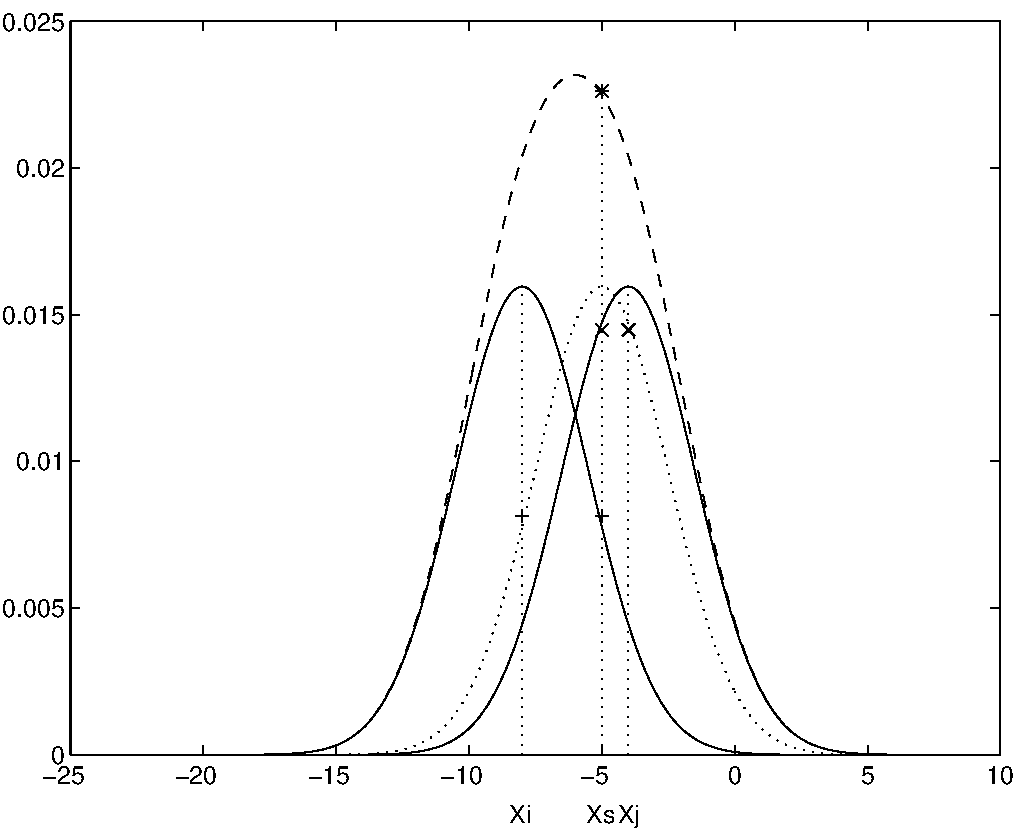
\includegraphics[height=6.5cm]{eijkel2}
  % \fbox{\rule{0pt}{0.8in} \rule{.95\linewidth}{0pt}}
  %\includesvg[inkscapelatex=false, width = 1\linewidth]{images/pipeline_frosting_largefont}
  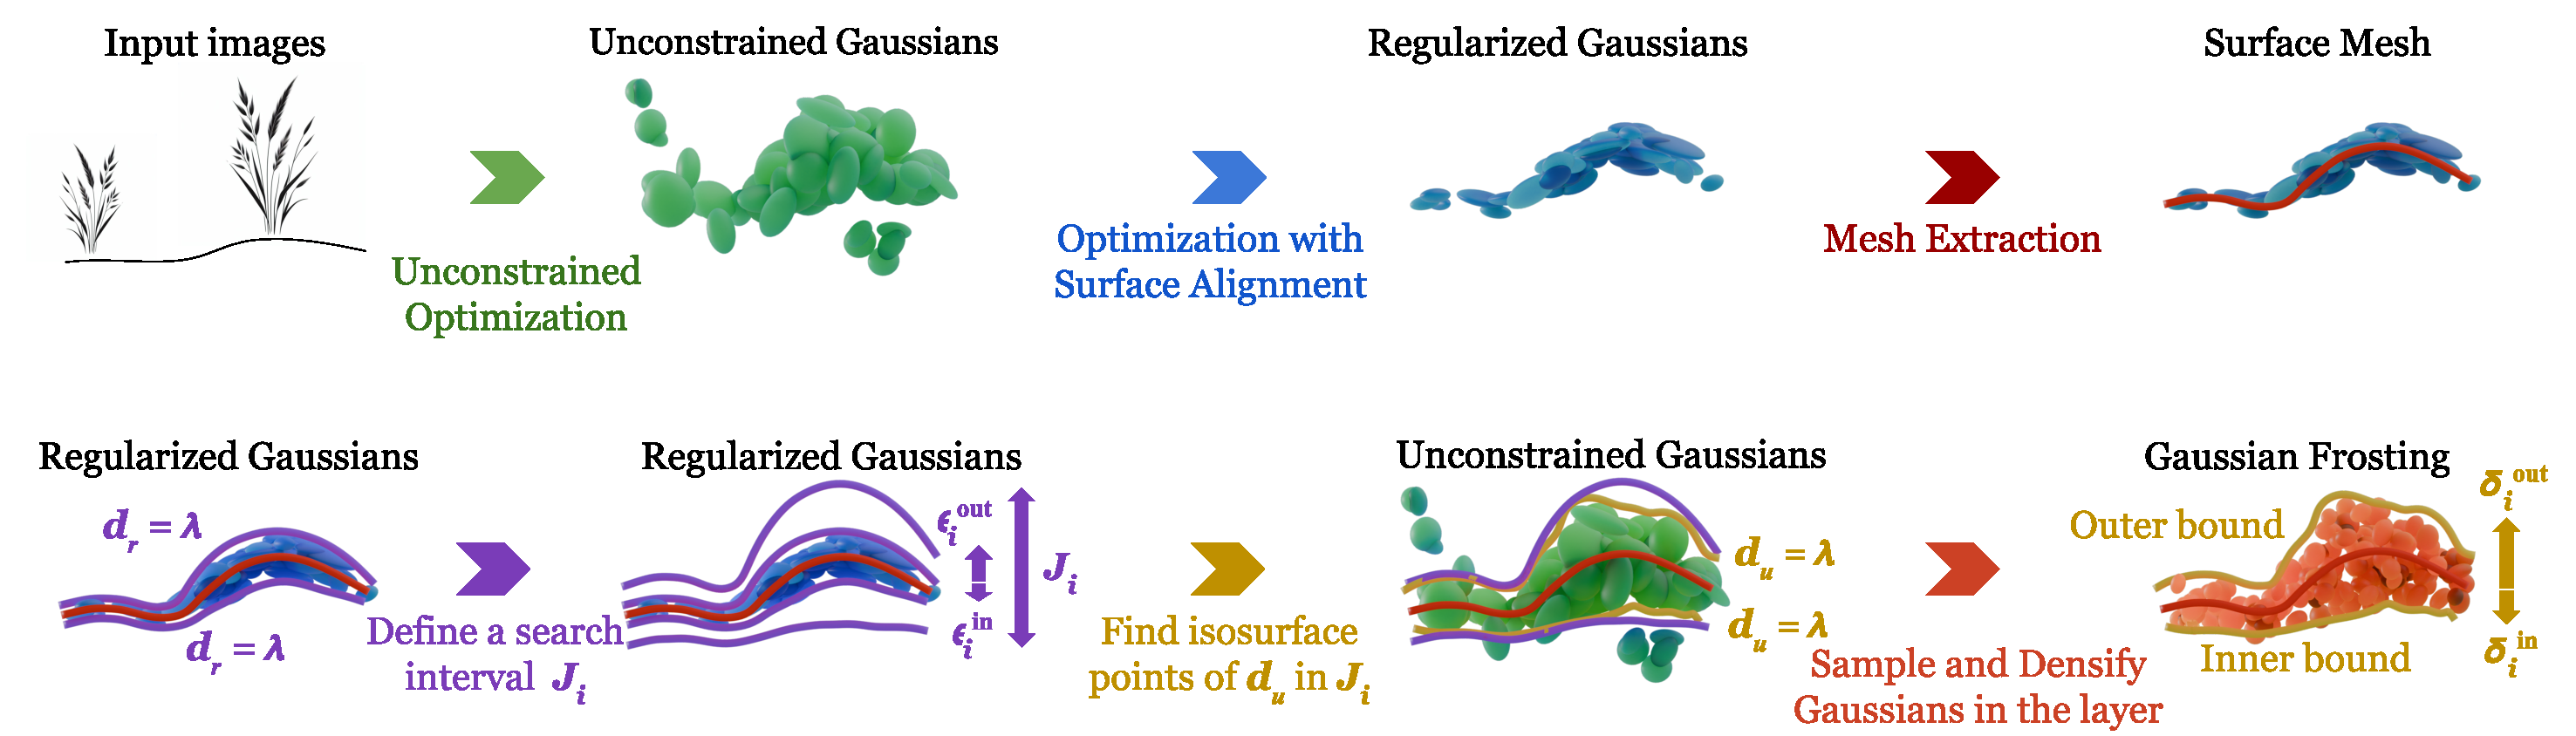
\includegraphics[width=\linewidth]{images/pipeline_frosting_largefont.pdf}
  \caption{
  \textbf{Creating a Layer of Gaussian Frosting.} To build our proposed Frosting representation, we start by optimizing a Gaussian Splatting representation using a rendering loss without any additional constraint, to let Gaussians position themselves. We refer to these Gaussians as \emph{unconstrained}. We then regularize these Gaussians to enforce their alignement with the surface, and extract a mesh that will serve as a basis for the Frosting. Next, we use the misalignment of surface-aligned Gaussians to identify areas where more volumetric rendering is needed, and we build search intervals $J_i$ around the mesh's vertices $\vec{v_i}$. Finally, we use the density function of the unconstrained Gaussians to refine the intervals, resulting in a Frosting layer. We finally sample a novel, densified set of Gaussians inside the layer.
}
  \label{fig:frosting-pipeline}
\end{figure}

\paragraph{Dense Video Caption Data Generation.} To generate high-quality video caption data, we established a complex data generation pipeline, as detailed in Figure~\ref{fig:video_caption_gen}. First, we used the Panda70M video captioning model to generate short captions for the videos. Then, we employed the image recaptioning model from CogView3~\citep{zheng2024cogview3} to create dense image captions for the frames within the videos. Subsequently, we used GPT-4 to summarize all the image captions to produce the final video caption. To accelerate the generation process from image captions to video captions, we fine-tuned a Llama 2 model~\citep{touvron2023llama} using the summary data generated by GPT-4~\citep{GPT4}, enabling large-scale video caption data generation. Additional details regarding the video caption data generation process can be found in Appendix~\ref{ap:video_caption_gen}.


\paragraph{Dense Video Caption Model Training.} To further accelerate the video caption generation process, we fine-tuned an end-to-end video understanding model, called CogVLM2-Caption, based on the CogVLM2-Video~\citep{CogVLM2-Video} and Llama 3~\citep{llama3modelcard}, using the dense caption data generated from aforementioned pipeline. We trained on 100k videos using a training cluster of 16 machines, each equipped with 8 A100 GPUs, for 10 epochs. This achieved the capability to generate dense video captions as described above through the pipeline method. Examples of video captions generated by our end-to-end model are shown in Appendix~\ref{ap:video_caption_example}. In Appendix~\ref{ap:v2v}, we also present some examples of video generation where a video is first input into CogVLM2-Caption to generate captions, which are then used as input for CogVideoX to generate new videos, effectively achieving video-to-video generation.



